\chapter{Endosymbiosis of mitochondria and chloroplasts (I)}

Most of life on Earth was composed of prokaryotes.
After some event eukaryotes were created.
The endosymbiotic theory explains the origin of mitochondria and chloroplasts in eukaryotes as well as the possible origin of eukaryotes \cite{endo, biomain}.

\section{Origin of eukaryotes}
Fossil evidence of cell bodies much bigger than prokaryotes have been dated to be around 1.5 BYA \cite{biomain}.
A nucleus, the organelle, has been found in the fossil cells, which suggests that evolution of eukaryotes from prokaryotic bodies.
It has also been noted that in prokaryotes have cell membrane \emph{invaginations} that may have led to the formation of the endoplasmic reticulum and the nucleus.

There are two models on the origin of eukaryotes \cite{endo}:

\begin{itemize}
    \item Eukaryotes have evolved from cell bodies with compartmentalization
    \item Eukaryotes have evolved from the process of endosymbiosis itself.
\end{itemize}

The first model says that a Gram-positive bacterium has lost its peplidoglycan cell wall.
Next, invaginations of the cell membrane enveloped the bacterial DNA forming a nucleus and formed the endoplasmic reticula.
The second model says that an peptidoglycan-less bacterium engulfed bodies around it which resulted in further compartmentalization within the cell forming a nucleus and endoplasmic reticula \cite{endo}.
Without the cell wall, there are two factors relating to cell growth worth noting: cell growth is possibly only limited by resource distribution efficiency, and there is a less restricted transfer of matter with the environment.

Following this development, Gram-negative energy-producing and/or photosynthetic bacteria may have entered the larger eukaryotic cell prototype described above.
The above is summarized by Figure~\ref{fig:endo} \cite{endo}.
In addition to the increase of mass of the eukaryotic cell, complex systems theory posits that there must be interaction between the engulfed cells and the host cell.
This interaction is called endosymbiosis.

\begin{figure}
    \centering
    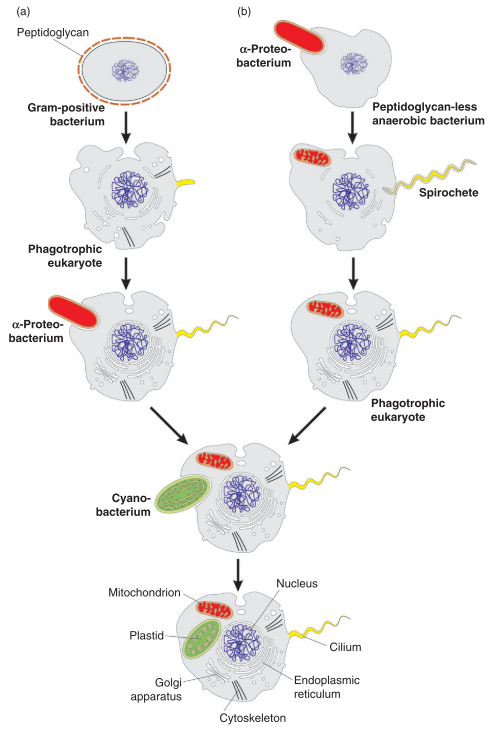
\includegraphics[scale=0.4]{endo}
    \caption{Two models of euakryote origin}
    \label{fig:endo}
\end{figure}

\section{Endosymbiosis of mitochondria}
The first step in the evolution of mitochondria was the manifestation of the complex interactions between the interior of the host cells and the engulfed bacteria.
Originally, following a traditional model of phagocytosis, the engulfed bacteria might have been thought as food for the eukaryotic cell, but that did not happen to be the case.
Somehow, the $\alpha$ -proteobacterium may have managed to disturb the digestion process of the host.
The fact that the symbiont has remained in the host allowed for sustainable symbiosis between the two organisms \cite{endo}.
This is a result of internal self-organization!

There are two processes in the symbiosis mentioned above: endosymbiotic gene transfer (EGT) from symbiont to host genome, and the transfer of transport proteins (translocons) on the membranes of the symbiont to the envelope surrounding it \cite{endo}.
The number of protein-encoding genes in present mitochondria are significantly less than those found in the hypothesized predecessors.
Some of these genes were either transferred to and incorporated with the host genome or may have been lost completely.
Again, the interacting organisms will have to adapt to such environment.
\citeA{endo} say that a possible reason for the decrease in number of such genes is to prevent complications from mutations.

The transfer of translocons improved the efficiency of protein transport between the host cell and the symbiont.
Moreover, such protein transport between mitochondria and the host has evolved from ``molecular tinkering'' \cite{endo}.
At this point the mitochondria have already been integrated with the host cell and are officially organelles.

\section{Endosymbiosis of chloroplasts}
Meanwhile, chloroplasts have been thought to evolve from cyanobacteria.
Similar processes, as with mitochondria, have occurred in the incorporation of the chloroplast.
However, there was more than one case this might have occurred since photosynthetic organisms don't belong to one group \cite{biomain}.

The secondary symbiosis events created chloroplasts with more than two envelope membranes \cite{endo}.
The explanation for these secondary symbiosis events is the endocytosis of green and red alga containing primary chloroplasts (\textit{ibid.}).
The evidence for this is well preserved by cryptophytes.
However, this begs the question: What happened to the nuclei and organelles of the green and red alga?
The question was not answered in both sources used above, but it can be hypothesized that a similar mechanism, as with the endosymbiosis of mitochondria with hosts:
the organelles of the symbiont are incorporated to the host,
EGT occurs between host and symbiont chloroplast and symbiont nucleus \cite{endo},
the mitochondria of the symbiont die off, possibly because the EGT between symbiont and host nucleus, making the organelle unlikely to survive without its needed proteins.

\paragraph{Evidences for endosymbiosis}
\citeA{biomain} notes that mitochondria and chloroplasts have circular DNA and that they divide through binary fission similar to bacteria.
This is proves that the organelles have bacterial origins!
A recent study has also shown that the method of binary fission of mitochondria (through protein ring pinching) is preserved in all eukaryotes, suggesting that there is only one event of mitochondrion endosymbiosis \cite{Kato2019}.
